\documentclass[../cheatSheetAlgoritmi.tex]{subfiles}
\begin{document}

\subsection{Esercitazione 10 - 08/04/20}
\textbf{Batterie - Greedy}
\begin{itemize}
	\item Siete a bordo di un'auto elettrica su un'autostrada. Entrate in autostrada al km 0 con la batteria carica e dovete uscire al km $L$.
	\item Prima che la vostra batteria si esaurisca (dopo $r$ km), dovete fermarvi in un'area di servizio e sostituirla con una batteria di ricambio.
	\item Sia $D[1...n]$ un vettore di interi, dove $D[i]$ è la distanza dell'area di servizio i-esima dall'inizio dell'autostrada.
	\item Scrivete un algoritmo che prenda in input $D,n,L$ e $r$ e restituisca il numero minimo di fermate necessarie per completare il viaggio. Discutere correttezza e complessità.
\end{itemize}
\begin{lstlisting}[caption=Batterie Greedy]
int maxSquare(int[] D, int n, int L, int r)
	% Ordino le distanza crescente le stazioni
	mergeSort(D, n)
	if r $==$ 0 or n $\leq$ 0 or D[n] + r < L then
		return -1
	int tot = 0
	int n_battery = 0
	int remaining = r - D[1]
	int i = 2
	while i $\leq$ n and tot $<$ L do
		% se con una batteria piena non riesco a raggiungerlo...
		if remaining $<$ 0 then
			return -1
		if remaining < D[i] - D[i-1]
			remaining = r - (D[i] - D[i-1])
			n_battery = n_battery + 1
		else
			remaining = remaining - (D[i] - D[i-1])
		tot = D[i] + remaining
		i = i + 1
	return n_battery
\end{lstlisting}
Il costo dell'algoritmo greedy proposto ha complessità $\mathcal{O}(n \log n)$ derivante dal fatto di dover riordinare per distanza crescente le stazioni di servizio. Supponiamo che $S[i...n]$ sia l'insieme contenente l'indice delle stazioni dove è necessario effettuare un cambio di batteria e che abbia cardinalità minore possibile (di fatto è la soluzione ottimale). Data $m = S[m]$ stazione più vicina all'ingresso dove è necessario fermarsi per cambiare la batteria, possono verificarsi i seguenti casi:
\begin{itemize}
	\item $m = S[i]$, quindi la stazione più vicina si trova in prima posizione e la soluzione ha cardinalità minima.
	\item $m \neq S[i]$ allora è possibile riordinare gli elementi di $S$ in modo da scambiare $S[i]$ con $m$ e ottenere una permutazione della soluzione con cardinalità minima.
\end{itemize}
\newpage
\begin{flushleft}
\textbf{Batterie - DP}
\end{flushleft}
Identico al caso precedente solo che...


\begin{itemize}
	\item Siano $D[1...n]$ e $C[1...n]$ due vettori di interi, dove $D[i]$ è la distanza dell'area di servizio i-esima dall'inizio dell'autostrada, e $C[i]$ è il costo di una nuova batteria nell'area $i$.
	\item Il costo totale del viaggio è dato dalla somma dei costi delle batterie sostituite per arrivare al km $L$.
\end{itemize}
\begin{lstlisting}[caption=Batterie DP]
int batterie(int[] D, int[] C, int n, int L, int r)
    int[] DP = new int[1..n]
    int minSoFar = $+\infty$
    mergeSort(D, C, n) % Ordino i due vettori per distanza dal kilometro 0
    if r $\geq$ D[1] then
        DP[1] = C[1]
    else
        DP[1] = $+\infty$
        if $r \geq L$ then
            minSoFar = 0
    for i = 2 to n do
        DP[i] = $+\infty$
        for j = i - 1 downto 1 do
            if D[j] + r $\geq$ D[i] then
                DP[i] = min(DP[i], DP[j] + C[i])
    for i = 1 to n do
        if D[i] + r $\geq$ L then
            minSoFar = min(minSoFar, DP[i])
    if minSoFar $==$ $+\infty$ then
        minSoFar = -1
    return minSoFar
\end{lstlisting}
La complessità della soluzione è $\mathcal{O}(n^2)$ in quanto per la costruzione di ogni cella della tabella delle soluzioni sono necessarie al più $\mathcal{O}(n)$ interazioni. \\
La correttezza della soluzione mostrata può essere provata nel seguente modo: \\
Sia DP[i] la tabella di programmazione dinamica che memorizza il costo minore necessario per il carburante avendo fatto rifornimento alla stazione i-esima, sempre che sia possibile arrivarci. L'equazione di ricorrenza è dunque la seguente:
\begin{equation*}
    DP[i]=\begin{cases}
        + \infty & \text{$\forall i \mid i < j \rightarrow D[j] + r > D[i]$ $\lor$ $i == 1$ $r < D[1]$} \\
        C[1] & \text{$i == 1 \land r \geq D[1]$}\\
        min(DP[j] + C[i])_{\forall j \mid j \leq i \land D[j] + r \leq D[i]} & \text{altrimenti}
    \end{cases}
\end{equation*} 

\textbf{Sottosequenza}\\
Una stringa $P$ è una supersequenza di una stringa $T$ se $T$ è una sotto-sequenza di $P$. Scrivere un algoritmo che restituisca la lunghezza della supersequenza comune minimale di due stringhe $P$,$T$, ovvero la più piccola supersequenza di entrambe le stringhe. Discutere correttezza e complessità dell'algoritmo proposto.\\
Esempio: L'unica supersequenza comune minimale di $AB$ e $BC$ è $ABC$, e la sua lunghezza è pari a 3.\\
Esempio: Esistono due supersequenze comuni minimali di $DAB$ e $DCB$, ovvero $DACB$ e $DCAB$, e la loro lunghezza è pari a 4.
\begin{lstlisting}[caption=Supersequenza comune minimale]
int supersequenzaComuneMinimale(ITEM[] S, ITEM[] T, int n, int m) 
    int[][] DP = new int[0..n][0..m]
    for i = 0 to n do
        DP[i][0] = i
    for j = 0 to m do
        DP[0][j] = j
    for i = 1 to n do
        for j = 1 to m do 
            if $P[i] == T[i]$ then 
                DP[i][j] = DP[i-1][j-1] + 1
            else
                DP[i][j] = min(DP[i-1][j], DP[i][j-1]) + 1
    return DP[n][m]
\end{lstlisting}
La complessità della soluzione proposta è $\mathcal{O}(nm)$ dovuta al popolamento della tabella delle soluzioni. \\
La correttezza è rappresentata dalla seguente formula ricorsiva: \\
Sia DP[i][j] il numero minimo di caratteri necessari per costruire una supersequenza dai prefissi P(i) e T(j), essa viene definita come segue: 


\begin{equation*}
    DP[i][j]=\begin{cases}
        0 & \text{$i == 0 \land j == 0$} \\
        j & \text{$i == 0 \land i \geq 0$} \\
        i & \text{$j == 0 \land i \geq 0$} \\
        DP[i-1][j-1] + 1 & \text{$P[i] == T[j]$} \\
        min(DP[i-1][j], DP[i][j-1] + 1) & \text{altrimenti} \\
    \end{cases}
\end{equation*}

I casi gestiti sono dunque:

\begin{itemize}
    \item Se le stringhe sono entrambe vuote l'unica supersequenza possibile è l'insieme vuoto.
    \item Se una delle due stringhe analizzata è vuota mentre l'altra non lo è allora la supersequenza comune minimale è quella che possiede dei caratteri. 
    \item Se i caratteri combaciano allora posso aggiungere il carattere considerato e considerare le stringhe con un carattere in meno entrambe
    \item Se i caratteri non combaciano allora cerco il minimo tra considerare o meno il carattere corrente di T e uno in meno di P e il viceversa, aggiungendo 1, ovvero il carattere considerato.
\end{itemize}
\textbf{Cammini Indipendenti}\\
Dato un grafo orientato $G= (V, E)$ e due vertici $s$, $t$ contenuti in $V$,descrivere un algoritmo che restituisca il numero totale di cammini $edge-disjoint$, ovvero in cui un arco può comparire al massimo in un cammino.
\begin{figure}[ht]
\caption{Edge-Disjoint Graph}
\centering
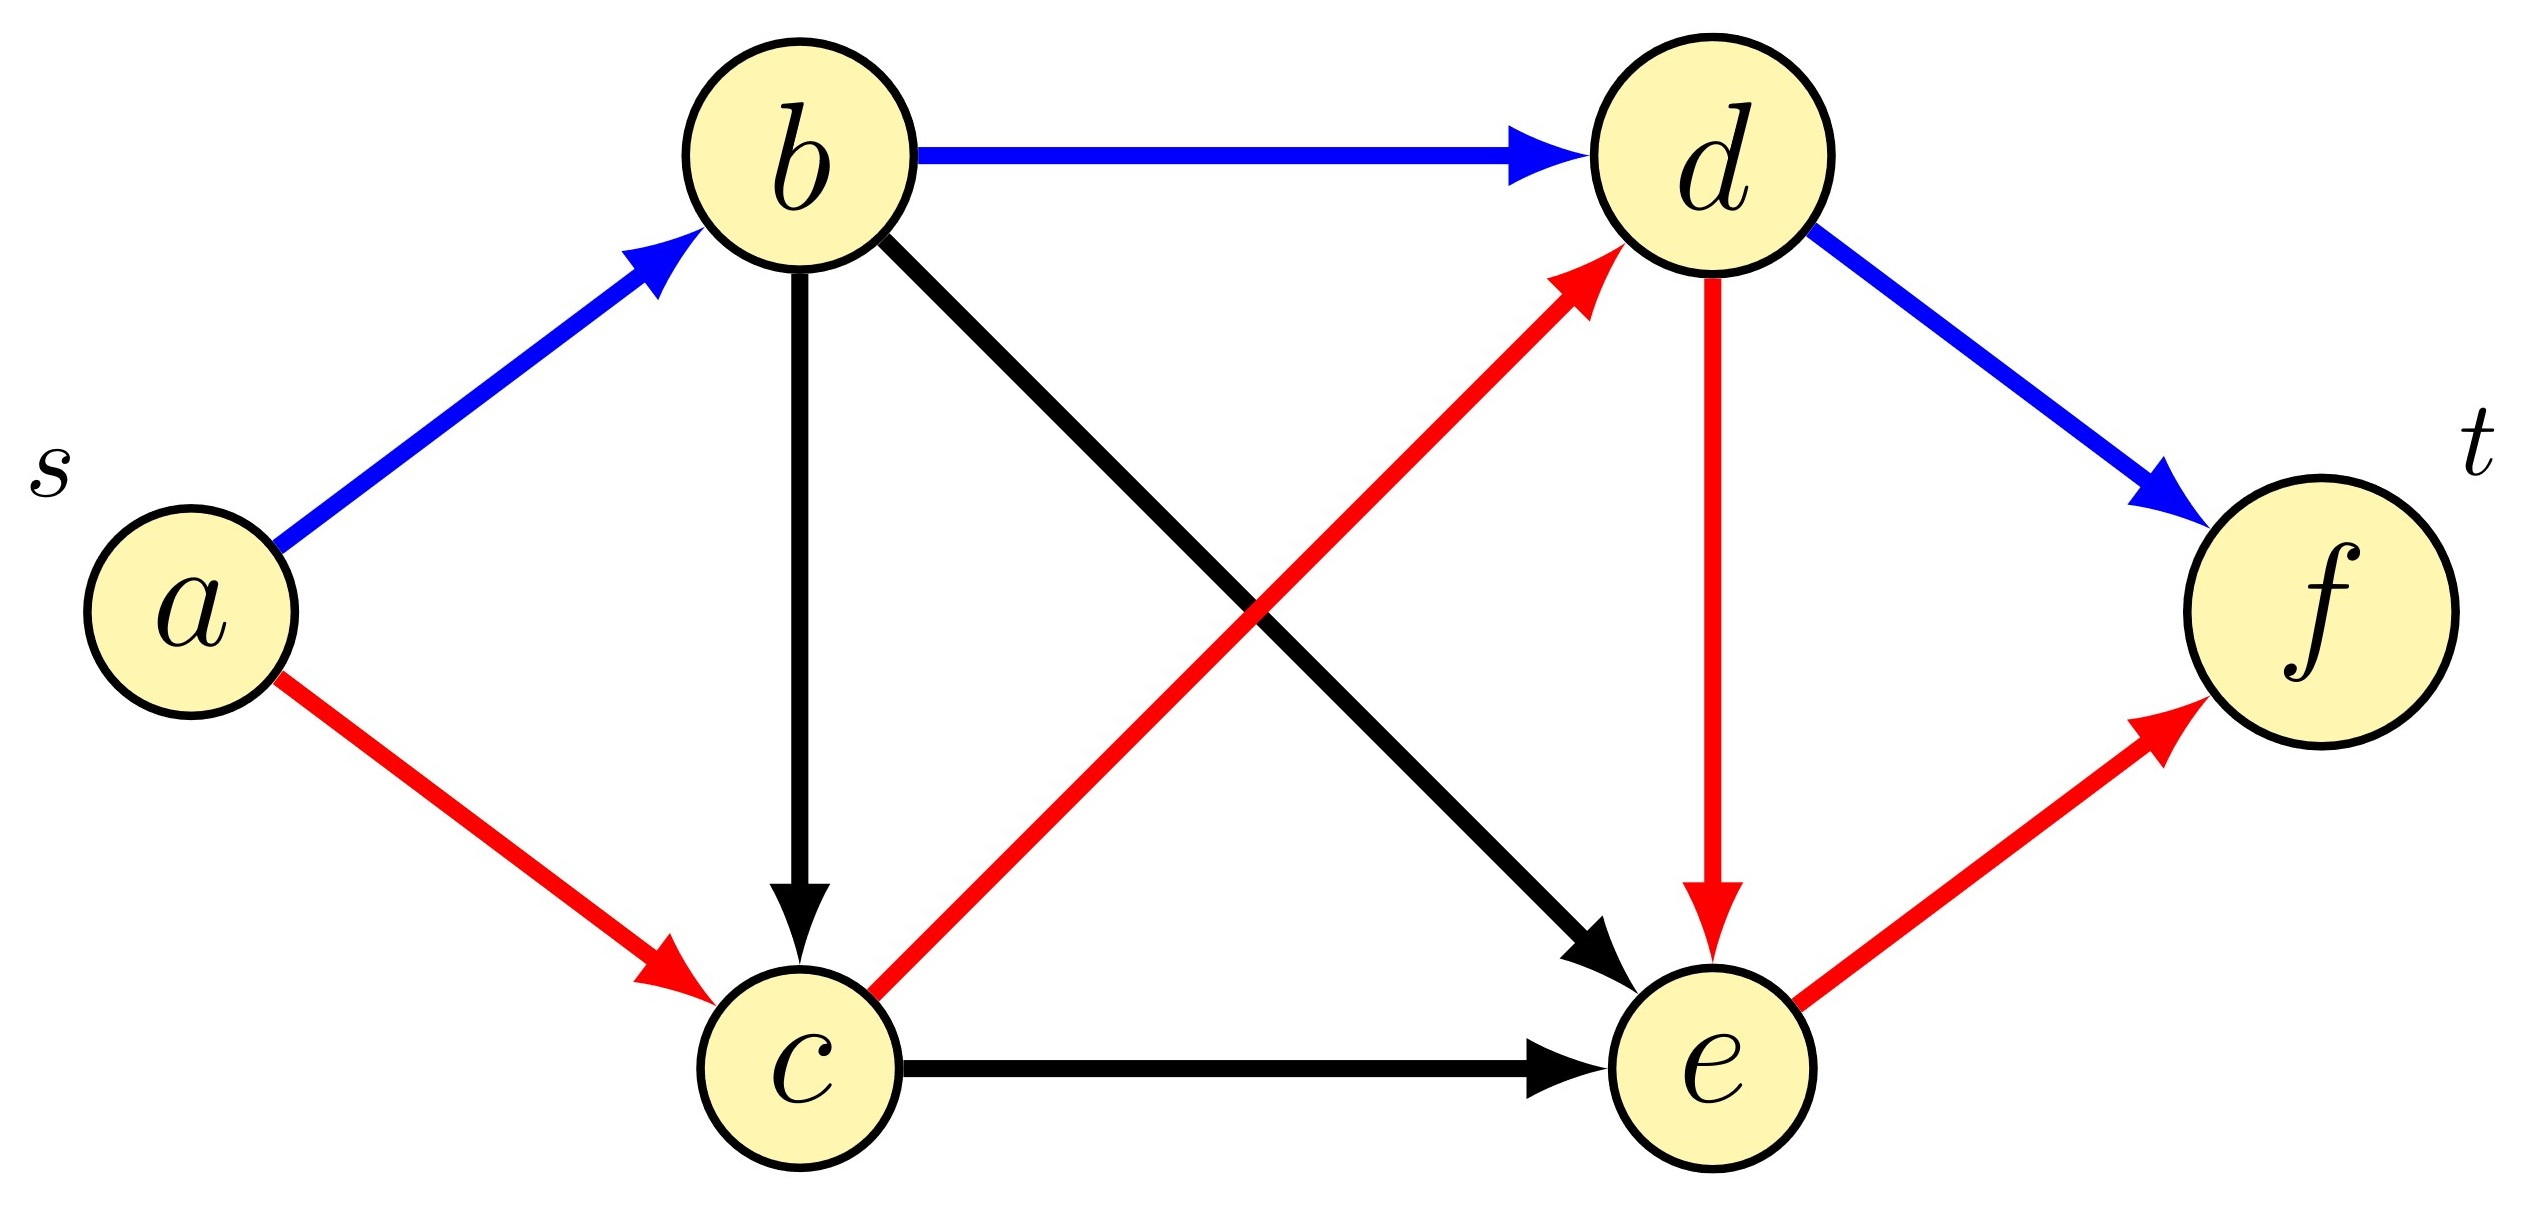
\includegraphics[width=0.5\textwidth]{../img/Locale_1.jpg}
\end{figure} \\
L'esercizio proposto non è altro che una Rete di Flusso $G(V, E, c, s, t)$ dove i nodi $s$ e $t$ sono rispettivamente supersorgente e superpozzo.\\
Visto che non è necessario aggiungere archi definiamo la funzione di capacità $c: V \times V \rightarrow R$  che associa ad ogni $(u, v) \in V$ il valore 1 in modo che venga percorso esattamente una e una sola volta.\\
Il numero di cammini edge-disjoint sarà dato dal flusso massimo $\mid f^* \mid$ associato a tale rete di flusso che è limitato superiormente da $\mathcal{O}(n)$ perché ci sono al più $(n-1)$ archi che escono dalla sorgente (o che entrano nel pozzo).
\newpage
\textbf{Torri di Controllo}
\begin{itemize}
    \item Si consideri un insieme di aerei $A=\{a_1,..., a_n\}$ e un insieme di torri di controllo $T=\{t_1,..., t_m\}$.
    \item In ogni istante, ogni aereo e ogni torre è dotato di coordinate geografiche $(a_{i.x}, a_{i.y})$ o/ $(t_{j.x}, t_{j.y})$. Ogni torre può gestire al più $L$ aerei, e ovviamente questi devono essere a portata radio $r$ dalla torre. 
    \item Descrivere un algoritmo che assegni ogni aereo ad una torre, rispettando i vincoli sulla distanza e sul carico. 
    \item Discutere correttezza e complessità.
\end{itemize}
Si costruisca una rete di flusso: $G(V, E, c, s, p)$ con le seguenti caratteristiche:
\begin{itemize}
    \item L'insieme $\mid V \mid$ di vertici è rappresentato dalla totalità di aerei e di torri, aggiungano inoltre due nodi, una supersorgente $s$ ed un superpozzo $p$.
    \item Aggiungiamo al grafo fornito i seguenti archi:
    \begin{itemize}
        \item Un arco tra la supersorgente ed ogni aereo
        \item Un arco tra ogni aereo e ogni torre
        \item Un arco tra ogni torre e il superpozzo
    \end{itemize}
    \item La funzione di capacità $c: V \times V \rightarrow R$ è così definita:
    \begin{itemize}
        \item Tutti, gli archi tra supersorgente e aereo devono avere una capacità pari a 1, in quanto un aereo può essere associato ad al massimo una torre
        \item La capacità sugli archi che connettono aereo e torre è così definita:
            \begin{equation*}
                c(a_{i}, t_{j})=\begin{cases}
                    1 & \text{$\mid \frac{a.y - t.y}{a.x - t.x} \mid \leq r$} \\
                    0 & \text{altrimenti}
                \end{cases}
            \end{equation*}
        \item Tutti gli archi tra torre e superpozzo devono avere capacità pari a $L$ in quanto ad ogni torre possono essere associati al più $L$ aerei
    \end{itemize}
\end{itemize}
Il flusso massimo $\mid f^* \mid$ associato a tale rete di flusso è limitato superiormente dal numero di aerei, in particolare: $\mid f^* \mid$ = $\mathcal{O}(n)$, il quale rappresenta la soluzione al problema dell'associazione massima possibile tra aerei e torri. \\
La complessità computazionale del calcolo della migliore associazione è data dal limite superiore di ordine più basso tra quello definito da Ford e Fulkerson e quello di Edmonds e Karp. \\
Possiamo dunque definire: 
\begin{itemize}
    \item $\mid V \mid$ = $2 + n + m$ dato che sono presenti la supersorgente, il superpozzo, gli aerei (n) e le torri (m).
    \item $\mid E \mid$ = $n + m + nm$ in quanto ogni aereo è connesso alla supersorgente, ogni torre al superpozzo e ogni aereo ad ogni torre.
\end{itemize}
Supponendo di aver rappresentato il grafo con liste di adiacenza posso definire la seguente complessità: \\
Il limite superiore per Ford e Fulkerson è dunque, nel caso peggiore, $\mathcal{O}((\mid V \mid + \mid E \mid) \mid f^* \mid)$ = $\mathcal{O}((2 + n + m + n + m + nm) n)$ = $\mathcal{O}((2 + 2n + 2m + nm) n)$ = $\mathcal{O}(2n + 2n^2 + 2nm + n^2m)$ = $\mathcal{O}(n^2m)$. \\
Mentre invece quello dettato dall'algoritmo di Edmonds e Karp vale: $\mathcal{O}(\mid V \mid (\mid E \mid)^2)$ = $\mathcal{O}((2 + n + m)(n + m + nm)^2)$ = $\mathcal{O}((2 + n + m)(n^2 + m^2 + n^2m^2 + 2nm + 2nm^2 + n^2m))$ = ... = $\mathcal{O}(n^2m^3)$.
La complessità per il calcolo del flusso massimo è dunque $\mathcal{O}(min(n^2m, n^2m^3)) = \mathcal{O}(n^2m)$.
\newpage
\end{document}